\chapter{Avaliação do WikiOlapBase}
\label{chap:avaliacao}

Terminado o desenvolvimento do WikiOlapBase foi realizada a avaliação da ferramenta segundo
a perspectiva dos usuários. Dois fatores são importantes na ferramenta desenvolvida, primeiro 
que ela seja adequada a utilização por parte do público alvo e segundo que ela permita a 
colaboração entre usuários \cite{barbosa2010}. Com o objetivo de verificar se esses 
fatores são atendidos foram realizados testes de usabilidade. Neste capítulo são discutidos a 
metodologia utilizada e os resultados encontrados.

\section{Metodologia de Avaliação}
\label{sec:metodologia-avaliacao}

Com intuito de avaliar a adequação de uso da ferramenta WOB, foi realizado um Teste de 
Usabilidade que consiste em um método de avaliação de interface que, além dos avaliadores,
envolve a participação de usuários e prevê as seguintes fases: Preparação, Execução e 
Análise \cite{barbosa2010}.

A fase de preparação é subdividida nas etapas de: (1) determinação dos objetivos do teste; 
(2) definição das tarefas que serão executadas; (3) seleção dos participantes; (4) 
considerações sobre os aspectos éticos; e (5) execução do teste piloto. Essas etapas geram 
artefatos que são posteriormente utilizados durante o passo de execução do Teste de 
Usabilidade. Dentre esses artefatos, incluem-se o \textit{Script} para apresentação do sistema, 
os  cenários de descrição das tarefas, o questionário de seleção dos participantes e o 
questionário pré-teste e o formulário de consentimento \cite{barbosa2010}.

É importante ressaltar que, além das tarefas que serão executadas pelos usuários, são 
definidas as métricas de usabilidade que serão observadas em cada execução. Para cada 
medida, são definidos os limites mínimos aceitáveis, os limites máximos possíveis e o 
valor almejado de usabilidade para cada métrica \cite{barbosa2010}.

A execução representa a fase em que ocorre a avaliação do sistema sob a perspectiva dos 
usuários. O avaliador conduz essa fase, efetuando as etapas de: (1) recebimento do usuário; 
(2) apresentação do sistema, conforme o \textit{Script} preparado; (3) consentimento formal dos 
usuários, utilizando para isso o termo de consentimento; (4) questionamento pré-teste, 
utilizando o questionário preparado; (5) observação das tarefas executadas pelos usuários e 
(6) a entrevista ou questionário pós-teste \cite{barbosa2010}.

Já na terceira fase do método, os dados coletados pelo avaliador são analisados. Nessa fase 
ocorre a verificação de cada uma das medidas de usabilidade, observadas durante a fase de 
execução, relacionando-as aos valores almejados durante a preparação. Nesse passo também 
são classificadas as gravidades dos problemas encontrados e possivelmente são discutidas as 
hipóteses relacionadas às causas dos problemas encontrados. Todos estes passos são 
posteriormente relatados em um relatório final do Teste de Usabilidade \cite{barbosa2010}.

Após elucidado a forma de condução do Teste de Usabilidade, é possível relatar como esse 
método foi conduzido para a avaliação da ferramenta WOB. Na fase de preparação, após 
estabelecido o objetivo do teste (i.e., avaliar a usabilidade e os mecanismos de 
colaboração do WOB), foram elaborados os artefatos que seriam utilizados durante as 
avaliações. São eles: o \textit{Script} da avaliação, o termo de consentimento de participação, 
os cenários de descrição das tarefas e a ficha de controle da avaliação. Esses artefatos 
podem ser visualizados no Apêndice 1.

Em relação às tarefas, é importante ressaltar que foram considerados os principais cenários de interação com o 
WOB, conforme segue: (T1) aprender a utilizar a ferramenta a partir das instruções presentes 
na seção de ajuda, (T2) enviar um conjunto de dados no formato CSV, (T3) observar o preview 
do conjunto de dados, (T4) preencher as informações básicas referentes ao conjunto de dados, 
(T5) definir \textit{tags} para as colunas do arquivo enviado e renomeá-las, (T6) definir uma 
hierarquia de dados dentro do conjunto enviado, (T7) enviar os metadados, (T8) 
verificar se o conjunto de dados foi incluído no repositório utilizando a 
ferramenta de busca, (T9) utilizar a API disponível para recuperar os dados que foram 
enviados e gerar visualizações e (T10) utilizar a API para cruzar dois conjuntos de 
dados distintos e gerar visualizações. 

A partir dessas tarefas foram definidos três cenários diferentes que envolvem uma ou mais 
delas, da seguinte forma: (C1) que envolve enviar um conjunto de dados e gerar uma 
visualização a partir do mesmo, para isso é necessário realizar as tarefas de T1 a T9; 
(C2) no qual deve-se enviar um conjunto de dados e fazer o cruzamento do mesmo com um 
conjunto de dados já existente no repositório para gerar uma visualização, para isso é 
preciso realizar as tarefas de T1 a T8 e T10; (C3) que envolve utilizar dois conjuntos de 
dados já existentes no repositório e gerar uma visualização a partir deles, logo é 
necessário realizar as tarefas T8 e T10. A fase de execução do teste de usabilidade do 
WOB contou com a participação de 6 usuários. Desses, 5 possuem formação na área de
computação (Engenharia de Computação ou Sistemas de Informação), o último possui 
formação em Engenharia Mecânica, porém todos atuam na área de desenvolvimento de software. 
Além disso, 4 possuem alguma experiência com um dos temas: análise de dados, visualização 
de dados ou mineração de dados

Para cada um dos cenários propostos foram realizados testes com dois usuários diferentes. 
Para cada tarefa executada por um usuário, o avaliador considerava o tempo gasto em sua 
execução e, além disso, observava e anotava como a tarefa era concluída (i.e., concluída 
sem erro, concluída com erro ou não concluída). Não era permitido ao longo da execução
que o avaliador respondesse a perguntas referentes a interface ou a alguma funcionalidade 
do WOB. Este tipo de pergunta seria respondida somente no período após cada tarefa, quando 
também seriam discutidas as dúvidas, dificuldades e sugestões dos usuários. 

Os testes de usabilidade, com os 6 usuários, ocorreram em um período de 3 dias, entre 27 de 
setembro de 2016 e 29 de setembro de 2016 sendo que cada um deles teve duração máxima de 
uma hora.

A partir dos dados obtidos, os resultados foram analisados de forma a caracterizar os 
indicadores de conclusão das tarefas pelos usuários; o tempo médio decorrido para cada uma 
das tarefas bem como o tempo médio total (i.e., tempo médio de conclusão de um cenário); e 
o grau de adequação do WOB aos princípios de usabilidade e colaboração. Através dessas 
medidas foi possível caracterizar a usabilidade e colaboração do WOB na perspectiva de 
seus usuários. Os resultados obtidos são discutidos a seguir.

\section{Discussão dos Resultados}
\label{sec:metodologia-resultados}

Em relação à execução das tarefas, o gráfico da Figura \ref{fig:avaliacao-tarefas} demonstra 
o percentual de conclusão de cada tarefa.

\begin{figure}[!htb]
    \centering
    \caption{Percentual de conclusão das tarefas pelos usuários}
    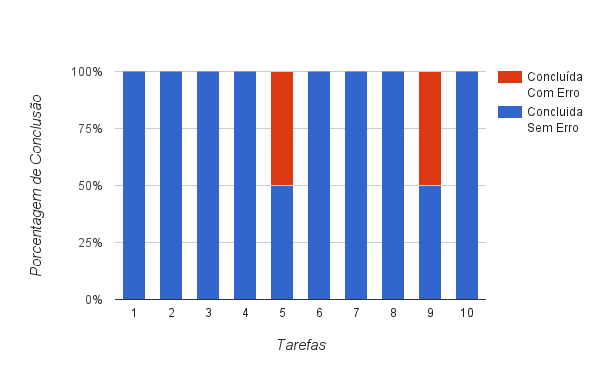
\includegraphics[width=1\textwidth]{./04-figuras/avaliacao-tarefas}
    \fonte{O Autor}
    \label{fig:avaliacao-tarefas}
\end{figure}

Através desse gráfico é possível observar que todas as tarefas foram concluídas pelos 
usuários, sendo que apenas 20\% foi concluída com erro, sendo a tarefa T5 concluída com 
erro por 2 usuários, e a tarefa T9 concluída com erro por 1 usuário.

A Tabela \ref{table:tempos-execucao}, por sua vez, apresenta o tempo decorrido para a execução de cada uma das 
tarefas pelos usuários e a média do tempo gasto pelos mesmos. Também são exibidos os 
tempos totais de execução das tarefas por cada usuário.

\begin{table}[!htb]
    \centering
    \caption{ Relação de tempo decorrido em minutos para cada uma das tarefas em cada teste de usabilidade}
    \label{table:tempos-execucao}
    \begin{tabular}{|p{1.5cm}|p{1.2cm}|p{1.2cm}|p{1.2cm}|p{1.2cm}|p{1.2cm}|p{1.2cm}|p{1.2cm}|p{1.5cm}|}
        \hline
        Tarefa & U1 & U2 & U3 & U4 & U5 & U6 & Total de Usuários & Tempo Médio \\
        \hline
        T1 & 01:07 & 03:09 & 01:56 & 01:20 & 00:00 & 00:00 & 4 & 01:53 \\
        \hline
        T2 & 00:18 & 00:31 & 00:27 & 00:20 & 00:00 & 00:00 & 4 & 00:24 \\          
        \hline
        T3 & 01:18 & 00:40 & 00:29 & 00:15 & 00:00 & 00:00 & 4 & 00:40 \\
        \hline
        T4 & 01:22 & 01:01 & 00:51 & 01:38 & 00:00 & 00:00 & 4 & 01:13 \\
        \hline
        T5 & 02:23 & 00:36 & 01:18 & 02:01 & 00:00 & 00:00 & 4 & 01:34 \\
        \hline
        T6 & 02:06 & 00:41 & 02:07 & 00:57 & 00:00 & 00:00 & 4 & 01:27 \\
        \hline
        T7 & 00:24 & 00:04 & 00:10 & 00:05 & 00:00 & 00:00 & 4 & 00:10 \\
        \hline
        T8 & 00:52 & 00:35 & 01:13 & 01:29 & 01:11 & 00:54 & 6 & 01:02 \\
        \hline
        T9 & 03:18 & 03:04 & 00:00 & 00:00 & 00:00 & 00:00 & 2 & 03:11 \\
        \hline
        T10 & 00:00 & 00:00 & 03:35 & 03:52 & 04:33 & 04:13 & 4 & 04:03 \\
        \hline 
        Total & 13:08 & 10:21 & 12:06 & 11:57 & 05:44 & 05:07 & - & - \\
        \hline   
    \end{tabular}
    \fonte{O Autor}
\end{table}


Os usuários U1 e U2 executaram o cenário C1, enquanto os usuários U3 e U4 executaram o 
cenário C2 e os usuários U5 e U6 executaram o cenário C3. Assim, também foi possível calcular
o tempo médio por cenário. Verificou-se que C1 possui um tempo médio de execução de 11 
minutos e 44 segundos, enquanto o tempo médio para concluir C2 é 12 minutos e 01 segundo, 
já o tempo médio para concluir C3 foi de 05 minutos e 25 segundos.

A tarefa T1 apresentou um tempo de execução similar entre a maioria dos usuários. Essa tarefa 
envolve acessar a página de instruções da ferramenta para aprender sobre seu funcionamento. 
Embora essa tarefa não tenha gerado dificuldades ou dúvidas, foi possível perceber que a 
maioria dos usuários prefere aprender a utilizar a ferramenta durante a própria execução. 
Isso explica o tempo discrepante que ocorreu, pois um usuário se mostrou mais interessado 
em entender as instruções de como utilizar a ferramenta antes de utilizá-la de fato. Já a 
tarefa T2 foi executada sem maiores problemas e sem grande variação de tempo entre os 
usuários.

A tarefa T3 apresentou uma pequena variação nos tempos de execução entre os usuários. 
Nessa tarefa os usuários deveriam verificar o conjunto de dados enviado a partir da 
funcionalidade “preview”. Durante a avaliação, 3 usuários reportaram dificuldades em 
localizar essa funcionalidade e, além disso, apresentaram sugestões de melhorias para 
a visibilidade dessa função. Embora esse tenha sido considerado um problema cosmético, 
as sugestões apontadas pelos usuários serão implementadas na próxima versão do WOB.

Já na execução da tarefa T4 não existiu nenhuma dúvida ou dificuldade. Uma tarefa que 
apresentou grande variação entre os tempos de execução foi a T5, além disso ela foi 
concluída com erro por 2 usuários. Nessa tarefa os usuários deveriam inserir tags para 
cada coluna do conjunto de dados enviado e renomear suas colunas. Os erros ocorreram por 
dois motivos: (1) não ficou claro a possibilidade de editar os nomes das colunas e a 
forma de fazer isso e (2) no processo para se adicionar uma tag é mostrada uma lista com 
tags já utilizadas anteriormente, não ficou claro, segundo os usuários, que era possível 
adicionar uma nova \textit{tag} que não existia nessa lista. Esse problemas serão corrigidos 
em versões futuras da ferramenta para melhorar a usabilidade do sistema.

A tarefa T6, embora tenha sido concluída sem erros por todos usuários, também apresentou 
problemas, o que fica claro com a variação entre os tempos de execução. Nessa tarefa 
deveria ser especificada uma hierarquia de dados dentro do conjunto de dados enviado. 
Dois usuários reportaram a falta de feedback ao se definir a hierarquia, ou seja, não era 
possível saber se a hierarquia havia sido salva ou não. Esse problema também será corrigido 
em uma futura versão da ferramenta.

Na execução das tarefas T7, T8 e T10 não ocorreram problemas. Já a tarefa T9 foi concluída 
com erro por um usuário. Nessa tarefa os usuários deveriam utilizar a API disponível para 
recuperar o conjunto de dados enviado, e a partir disso gerar uma visualização. Uma possível 
explicação, para o erro cometido nessa tarefa, é a falta de experiência do usuário na 
utilização de \textit{web services}. Vale ressaltar que embora o objetivo da ferramenta 
seja permitir sua utilização mesmo por parte de usuários inexperientes, o projeto prevê uma 
segunda fase na qual será desenvolvida uma ferramenta de visualização de dados que irá 
consumir a API desenvolvida, logo isso não deverá ser um problema para usuários menos 
experientes no futuro pois o acesso direto a API não será necessário.

Conforme mencionado anteriormente, depois de executadas as tarefas, cada usuário avaliou a 
ferramenta sob a perspectiva dos 07 princípios de usabilidade \cite{nielsen1994usability}, 
além dos 02 princípios de colaboração definidos especificamente para essa ferramenta, são 
eles: (1) colaboração passiva e (2) colaboração ativa . Para que seja realizada uma análise 
mais assertiva as respostas foram separadas de acordo com o cenário para o qual cada usuário 
foi submetido, dessa forma a Figura \ref{fig:avaliacao-cenario1} sumariza as respostas para os 
usuários que realizaram o cenário C1, a Figura \ref{fig:avaliacao-cenario2} para os usuários 
que realizaram o cenário C2 e a Figura \ref{fig:avaliacao-cenario3} para os usuários que 
realizaram o cenário C3

O termo colaboração passiva se refere a utilizar um conjunto de dados já existente, ou 
seja, o grau com que o sistema permite que usuários utilizem conjuntos de dados que foram 
enviados por outros usuários, já o termo colaboração ativa se refere a enviar um conjunto 
de dados para outra pessoa utilizar, ou seja, o grau com que o sistema incentiva a 
colaboração entre usuários, mostrando que ao enviar um conjunto de dados ele estará 
disponível para qualquer um utilizar.

\begin{figure}[!htb]
    \centering
    \caption{Grau de adequação do WOB por princípio de usabilidade e colaboração na visão dos usuários - Cenário C1}
    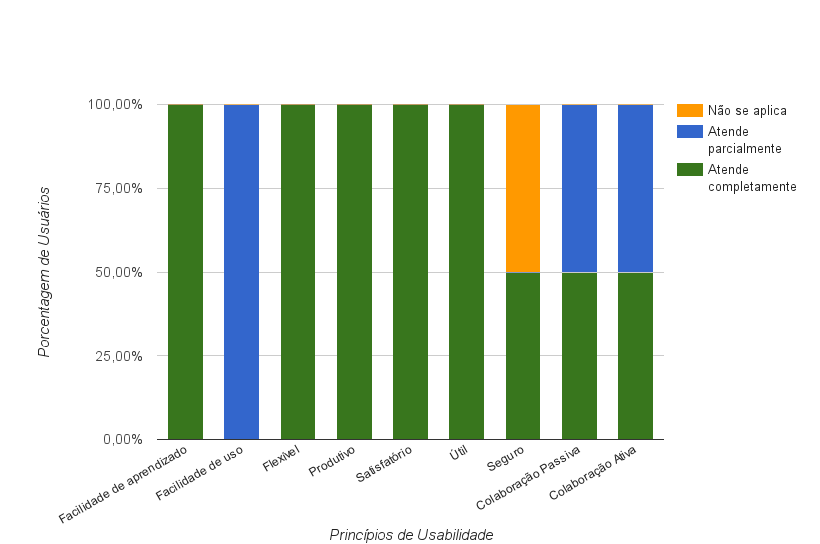
\includegraphics[width=0.8\textwidth]{./04-figuras/avaliacao-cenario1}
    \fonte{O Autor}
    \label{fig:avaliacao-cenario1}
\end{figure}

\begin{figure}[!htb]
    \centering
    \caption{Grau de adequação do WOB por princípio de usabilidade e colaboração na visão dos usuários - Cenário C2}
    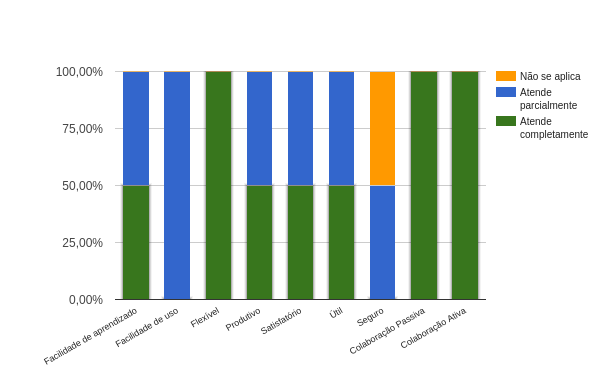
\includegraphics[width=0.8\textwidth]{./04-figuras/avaliacao-cenario2}
    \fonte{O Autor}
    \label{fig:avaliacao-cenario2}
\end{figure}

\begin{figure}[!htb]
    \centering
    \caption{Grau de adequação do WOB por princípio de usabilidade e colaboração na visão dos usuários - Cenário C3}
    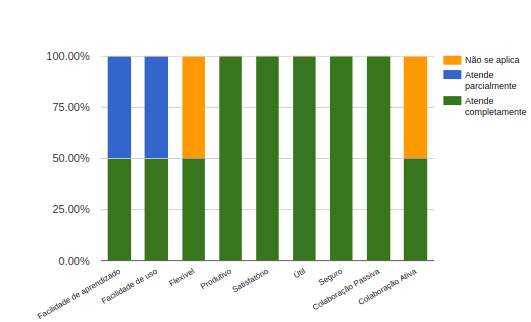
\includegraphics[width=0.8\textwidth]{./04-figuras/avaliacao-cenario3}
    \fonte{O Autor}
    \label{fig:avaliacao-cenario3}
\end{figure}


Através dos dados apresentados é possível observar que nos três cenários nenhum princípio 
foi julgado como “não atende”, na perspectiva dos usuários, ou seja, para todos os usuários 
todos os princípios são atendidos ou não são aplicáveis. Foi possível perceber que para 
66.67\% dos usuários o WOB atende completamente o princípio de facilidade de aprendizado, no 
entanto para apenas 16.67\% o princípio de facilidade de uso é atendido completamente. Isso 
mostra que na visão desses usuários, embora, inicialmente, o WOB não apresente uma fácil 
utilização, aprender como utilizá-la é uma tarefa simples. 

Pode-se notar também, que três princípios foram julgados como não aplicáveis. No cenário 
C1 e C2 foi o princípio “Seguro”, já no cenário C3 foram os princípios “Flexível” e 
“Colaboração Ativa”. Os usuários julgaram que o princípio “Seguro” não se aplica pois a 
ferramenta é aberta, permitindo sua utilização por qualquer pessoa. Já para os casos dos 
princípios “Flexível” e “Colaboração Ativa” os usuários julgaram que estes não se aplicam 
devido ao cenário que foram expostos. O cenário C3 envolve apenas a busca por dois 
conjuntos de dados já existentes no repositório e a utilização da API para o cruzamento 
desses dados, não envolvendo portanto caminhos alternativos ou o envio de conjuntos de 
dados para a utilização por outros usuários, isso explica a interpretação dos usuários 
ao responderem que os princípios não se aplicam.

Embora existam melhorias a serem implementadas, tanto que foram identificadas durante o 
teste, quanto aquelas que já estavam planejadas para futuras versões (ver lista de 
melhorias no Apêndice 2), conclui-se que a ferramenta WOB é adequada ao uso. Isso é 
corroborado pela fala dos usuários ao longo dos testes, que aprovaram a idéia por trás da 
ferramenta bem como seu fluxo de execução. 
